\documentclass{beamer}
\mode<presentation>
\usetheme{Madrid}
\usecolortheme{crane}

\usepackage{tikz}
\usepackage{epic}
\usepackage{tikz-qtree}
\usepackage{linguex}
\usepackage[normalem]{ulem}
\usepackage{tikz-dependency}
\usepackage{colortbl}
\usepackage{xcolor}
\definecolor{darkgreen}{rgb}{0,0.3,0}
\definecolor{darkblue}{rgb}{.05,.05,.30}
\definecolor{lightgrey}{rgb}{0.65,0.65,0.65}
\usepackage{tikzsymbols}
\usepackage{amsmath}
\usepackage{multirow}

\newcommand{\norm}[1]{\left\lVert#1\right\rVert}
\newcommand{\remph}[1]{\textbf{\color{red} #1}}


\DeclareMathOperator*{\argmax}{argmax}


\title[LT2222 lecture 2]{LT2222 Machine learning for NLP: introduction, Winter 2021}
\subtitle{Lecture 2: Vectors and matrices; classification; dimensionality reduction}
\author[Sayeed]{Asad Sayeed}
\institute[Gothenburg]{University of Gothenburg}
\date{}

\setbeamertemplate{navigation symbols}{}

\newcommand{\placard}[1]{
  \begin{frame}
    \begin{center}
      \huge
      \textbf{#1}
    \end{center}
  \end{frame}
}

\newcommand{\pagestep}[2]{
  \begin{frame}[t]
    \begin{minipage}[t][0.26\textheight][t]{\textwidth}
      \begin{center}
        \huge
        \textbf{#1}
      \end{center}
    \end{minipage}
    
    \begin{minipage}[t][0.7\textheight][c]{\textwidth}
      \begin{center}
        \includegraphics[height=0.83\textheight]{#2}
      \end{center}
    \end{minipage}
  \end{frame}
}

\newcommand{\pagestepalt}[2]{
  \begin{frame}[t]
    \begin{minipage}[t][0.26\textheight][t]{\textwidth}
      \begin{center}
        \huge
        \textbf{#1}
      \end{center}
    \end{minipage}
    
    \begin{minipage}[t][0.7\textheight][c]{\textwidth}
      #2
    \end{minipage}
  \end{frame}
}

%% \newcommand{\pagestepaltfragile}[2]{
%%   \begin{frame}[fragile][t]
%%     \begin{minipage}[t][0.26\textheight][t]{\textwidth}
%%       \begin{center}
%%         \huge
%%         \textbf{#1}
%%       \end{center}
%%     \end{minipage}
    
%%     \begin{minipage}[t][0.7\textheight][c]{\textwidth}
%%       #2
%%     \end{minipage}
%%   \end{frame}
%% }


\begin{document}
\makeatletter
\setbeamertemplate{footline}
{
  \leavevmode%
  \hbox{%
  \begin{beamercolorbox}[wd=.333333\paperwidth,ht=2.25ex,dp=1ex,center]{author in head/foot}%
    \usebeamerfont{author in head/foot}\insertshortauthor\expandafter\beamer@ifempty\expandafter{\beamer@shortinstitute}{}{~~(\insertshortinstitute)}
  \end{beamercolorbox}%
  \begin{beamercolorbox}[wd=.333333\paperwidth,ht=2.25ex,dp=1ex,center]{title in head/foot}%
    \usebeamerfont{title in head/foot}\insertshorttitle
  \end{beamercolorbox}%
  \begin{beamercolorbox}[wd=.333333\paperwidth,ht=2.25ex,dp=1ex,right]{date in head/foot}%
    \usebeamerfont{date in head/foot}\insertshortdate{}\hspace*{2em}
%    \insertframenumber{} / \inserttotalframenumber\hspace*{2ex} 
    \insertframenumber{}\hspace*{2ex}
    \hspace*{6ex}
  \end{beamercolorbox}}%
  \vskip0pt%
}
\makeatother


\begin{frame}
  \titlepage
\end{frame}

\pagestepalt{Today's agenda:}{
  \begin{enumerate}
  \item Classification concepts review
  \item Dimensionality reduction
  \item Vector-space classification
  \item Maximum entropy
  \end{enumerate}
}

\placard{Part 1: Classification: what it's for}


\pagestepalt{What classifiers do\ldots}{

  \begin{itemize}
    \item Given an object, assign a category.
    \item Such tasks are pervasive in NLP.
  \end{itemize}

}


\pagestepalt{Example: classification of documents}{

\begin{itemize}
\item ``Classic'' sentiment analysis: develop a program that groups customer reviews into positive
  and negative classes (given the text only)
\begin{center}

\includegraphics[scale=0.4]{images/amazon}
\end{center}

\pause
\item other examples:\pause
  \begin{itemize}
    \item Reuters, $\sim$ 100 hierarchical categories\pause
    \item Classification according to a library system (LCC, SAB)\pause
    \item \ldots by target group (e.g. CEFR readability) or some
      property of the author (e.g. gender, native language)
  \end{itemize}
\end{itemize}

}



\pagestepalt{Example: disambiguation of word meaning in context}{

\emph{A woman and child suffered minor injuries after the car they were riding in crashed into a \remph{rock} wall Tuesday morning.}\pause

\begin{itemize}
\item what is the meaning of \emph{rock} in this context?\pause
  \begin{center}
\begin{center}
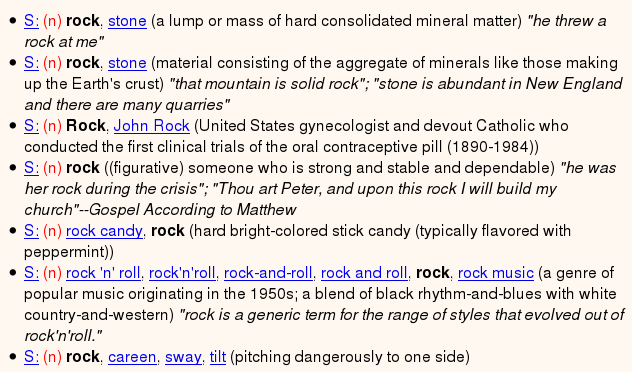
\includegraphics[scale=0.35]{images/rock}
\end{center}
  \end{center}
\end{itemize}
}


\pagestepalt{Example: classification of grammatical relations}{

\begin{center}
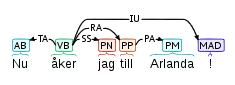
\includegraphics[scale=0.5]{images/arlanda}
\end{center}\pause

\begin{itemize}
\item What is the grammatical relation between \emph{\aa{}ker} and \emph{till}?\pause
  \begin{itemize}
    \item e.g. subject, object, adverbial, \ldots
  \end{itemize}
\end{itemize}
}


\pagestepalt{Example: classification of discourse relations}{

\emph{Mary had to study hard. Her exam was only one week away.}

\pause

\begin{itemize}
  \item What is the discourse/rhetorical relation between the two sentences?\pause
  \begin{itemize}
    \item e.g. IF, THEN, AND, BECAUSE, BUT, \ldots
  \end{itemize}
\end{itemize}

}



\pagestepalt{Features for classification}{

\begin{itemize}
  \item To be able to classify an object, we must describe its properties: \remph{features}\pause
  \item Useful information that we believe helps us tell the classes apart.\pause
  \item This is an art more than a science.\pause

  \item Examples:\pause
    \begin{itemize}
      \item In document classification, typically the \remph{words}\pause
      \item \ldots But also stylistic features such as sentence
        length, word variation, syntactic complexity
    \end{itemize}

\end{itemize}

}


\pagestepalt{Representation of features}{

\begin{itemize}
  \item depending on the task we are trying to solve, features may be
    viewed in different ways\pause
  \item \remph{bag of words}: \texttt{["I", "love", "this", "film"]} \pause
  \item \remph{attribute--value pairs}: \texttt{\{"age"=63, "gender"="F", "income"=25000\}}\pause
  \item \remph{geometric vector}: \texttt{[0, 0, 0, 0, 1, 0, 0, 2, 0,
      0, 1]}

%  \item in this lecture and in the assignments, we will use the bag of
%    words representation
\end{itemize}

}

\placard{Part 2: Dimensionality reduction}

%% \pagestepalt{Memory is cheap, right?}{
%%   But data always finds a way to exceed it.\pause
%%   \begin{itemize}
%%   \item Depending on how you define the contexts, can be mi
%%   \end{itemize}
%% }


%stuff on LSA, word2vec, etc.

\pagestepalt{The power of dimensionality reduction}{
  The count-based (e.g. word count)  vector-spaces are very high-dimensional.\pause
  \begin{itemize}
  \item Any ``respectable'' space will have a dimensionality that is 
    lexicon scale (at least!). \pause
  \item But since the dimensions are labelled by linguistic features, 
    those features have interrelationships. \pause  
  \item What we need: a way to ``compress'' feature dimensions so that
    relationships are revealed.\pause
  \end{itemize}
  Dimensionality reduction $==$ clustering features that have
  ``latent'' relationships $==$ ``prediction''.\pause
  \begin{itemize}
  \item e.g., a particular class of verb may be partly associated with 
    particular negative polarity items (``any'', ``nobody'', etc).\pause  
  \item Downside: often lose all direct human interpretability of
    ``reduced'' feature space.
  \end{itemize}
}

\pagestepalt{Common dimensionality reduction}{
  There are very many ways to generate lower-dim spaces.\pause Examples:
  \begin{itemize}
  \item Feature selection approaches: test subsets of features for
    e.g. information-theoretic properties.\pause (Why not?)\pause
  \item Tensor factorization approaches: 
    \begin{itemize}
    \item Factor the vector space into multiple smaller-dimensional matrices.
    \item Select rows/columns by importance heuristic
    \item Examples: Latent Semantic Indexing, Principal Component Analysis
    \end{itemize}\pause
  \item Discriminative training/machine learning approaches
    \begin{itemize}
    \item Iteratively update smaller-dimensional vectors.
    \item Update based on ability to reconstruct ``objective'' data.
    \item Examples: autoencoders, deep learning
    \end{itemize}
  \end{itemize}
}

\pagestepalt{Latent semantic analysis}{
  Factoring via Singular Value Decomposition (SVD) -- very widely used. 
  Based on Wikipedia:
  \begin{center}
    \includegraphics<1>[width=0.9\textwidth]{svd-s.pdf}
    \includegraphics<2>[width=0.9\textwidth]{svd-2-s.pdf}
    \includegraphics<3>[width=0.9\textwidth]{svd-3-s.pdf}
    \includegraphics<4>[width=0.9\textwidth]{svd-4-s.pdf}
    \includegraphics<5>[width=0.9\textwidth]{svd-5-s.pdf}
    \includegraphics<6>[width=0.9\textwidth]{svd-6-s.pdf}
    \includegraphics<7>[width=0.9\textwidth]{svd-7-s.pdf}
    \includegraphics<8>[width=0.9\textwidth]{svd-8-s.pdf}
  \end{center}
  \uncover<8>{
  The $\sigma$ are ranked, simply cut off dimensions at low-enough $\sigma$.\\
  %All vectors are similarly reduced so can multiply again to get low-dim
  %matrix.\\
  Dimensions represent ``fuzzy'' clusters, not directly interpretable.
  }
}

\pagestepalt{Latent semantic analysis}{
  Things to keep in mind with SVD/LSA.\pause
  \begin{itemize}
  \item Computationally intensive
    \begin{itemize}
    \item Computed using approximation and numerical tricks.  Still needs a lot of memory.
    \item Alternative approaches, e.g. ``Random Indexing''.
    \end{itemize}\pause
  \item Solutions not unique -- can get different answers from different approximations.\pause
  \item FYI: APIs both in numpy and sklearn.
  \end{itemize}
}

\placard{Part 3: Vector-space classification}


\pagestepalt{Classification}{
  \begin{columns}[T]
    \begin{column}{0.49\textwidth}
      \begin{center}
        \includegraphics<1>[width=0.9\textwidth]{reg2.pdf}
        \includegraphics<2>[width=0.9\textwidth]{reg3.pdf}
        \includegraphics<3-4>[width=0.9\textwidth]{linsep1.pdf}
        \includegraphics<5>[width=0.9\textwidth]{linsep2.pdf}                
      \end{center}
    \end{column}

    \begin{column}{0.49\textwidth}
      But sometimes we want a different hypothesis.
      \only<2-3>{
        \begin{itemize}
        \item<2-3> Instead, we're not looking for the response, but the \textbf{class}.\pause
        \item<3-3> Which means we're looking for an entirely different hyperplane.
        \end{itemize}
      }
      \only<4-5>{
        \begin{itemize}
        \item<4-5> In fact, we're trying to find $\mathbf{w}$ and $b$ such that
          \begin{block}{}
            \[
            f(\mathbf{x}) =
            \begin{cases}
              1 & \text{if } \mathbf{w} \cdot \mathbf{x} + b > 0 \\
              0 & \text{otherwise}
            \end{cases}
            \]
          \end{block}
        \item<5-5> And then we can decide the hyperplane
          $y = \mathbf{w} \cdot \mathbf{x} + b$.
        \end{itemize}
      }
    \end{column}
  \end{columns}
}



\pagestepalt{The perceptron: a very simple neural network}{
  {\small (from Wikipedia)}
  \begin{center}
    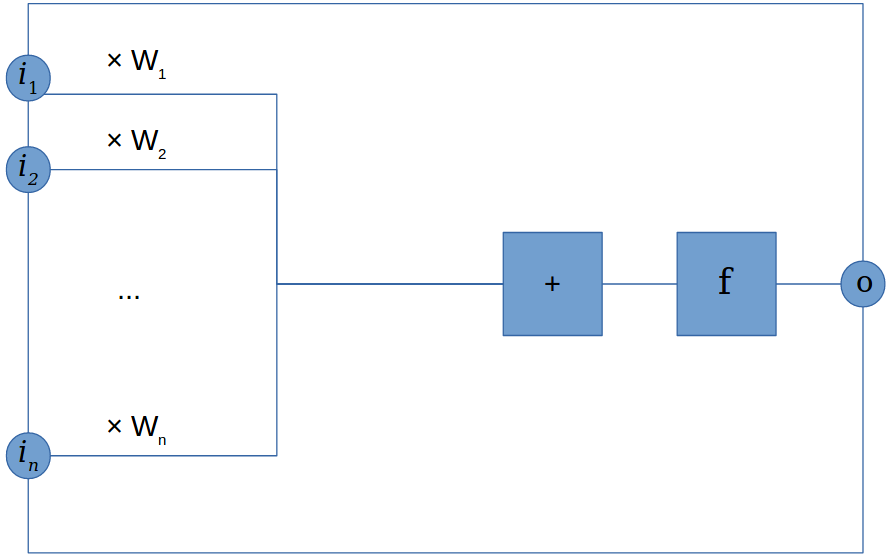
\includegraphics[width=0.45\textwidth]{perceptron-cropped.png}
  \end{center}\pause
  \begin{itemize}
  \item Each instance vector $\mathbf{x}$'s values are fed as inputs
    $i$ to the network.\pause
  \item Feature function $f$ is applied (remember: 1 or 0 output).\pause
  \item Weights adjusted based on output correctness.
  \end{itemize}
}

\pagestepalt{Perceptron algorithm (roughly)}{ Initialize weights
  $\mathbf{w}$ and bias (usually to (close to) 0). \\ Given $n$
  feature vectors $\mathbf{x}$ and corresponding ``ground truth'' values $d$, for vector $\mathbf{x}_i$:
  \begin{itemize}
  \item Calculate $f(\mathbf{x})$ as 1 or 0 using $\mathbf{w} \cdot \mathbf{x}_i + b$.
  \item Update weights as $\mathbf{w} \leftarrow \mathbf{w} + (d_i - f(\mathbf{x_i}))\mathbf{x_i}$.
  \item Move to next $\mathbf{x}$ feature vector, cycling through vectors until
    \alert{convergence}.
  \end{itemize}
  (There is a theoretical upper bound on how many iterations are required
  to converge.)
}

\pagestepalt{Perceptron limitations}{
  \begin{columns}[T]
    \begin{column}{0.49\textwidth}
      \begin{center}
        \includegraphics<1>[width=0.9\textwidth]{linsep2.pdf}
        \includegraphics<2->[width=0.9\textwidth]{freedom.pdf}
      \end{center}
    \end{column}

    \begin{column}{0.49\textwidth}
      What line do you choose?\pause
      \begin{itemize}
      \item Many are possible, perceptron does not fit one reliably.\pause
      \item Why is this a problem?
      \end{itemize}
    \end{column}
  \end{columns}
}

\pagestepalt{Perceptron limitations}{
  \begin{columns}[T]
    \begin{column}{0.49\textwidth}
      \begin{center}
        \includegraphics<1>[width=0.9\textwidth]{linsep2.pdf}
        \includegraphics<2->[width=0.9\textwidth]{linsep3.pdf}
      \end{center}
    \end{column}

    \begin{column}{0.49\textwidth}
      Our picture so far has been very convenient.\pause
      \begin{itemize}
      \item What if a point of one class was surrounded by points of the other
        class?\pause
      \item Perceptrons \alert{don't converge} if space is not \textbf{linearly separable}.\pause
      \item Setting a ``tolerance'' doesn't help much -- need more
        complex variant.
      \end{itemize}
    \end{column}
  \end{columns}
}

\pagestepalt{Support vector machines}{
  Support vector machines (SVMs) find hyperplanes in the same sense as
  perceptrons. But they're more versatile.\pause
  \begin{itemize}
  \item Linear SVM -- not only find a separating hyperplane, but
    also the ``optimal'' hyperplane, given some tolerance.\pause
  \item Nonlinear SVM -- Same as linear SVM, but find hyperplanes that
    work for linearly \alert{inseparable} data.\pause
  \item The algorithms are more advanced than a perceptron: quadratic
    programming, gradient descent -- we'll get into gradient descent
    probably in a later class.\pause
  \end{itemize}
  But what is a support vector?
}

\pagestepalt{Hard-margin linear SVM}{
  \begin{columns}[T]
    \begin{column}{0.49\textwidth}
      \begin{center}
        \includegraphics<1>[width=0.9\textwidth]{freedom.pdf}
        \includegraphics<2->[width=0.9\textwidth]{hard-margin.png}
        \only<2->{\\ \small (from Wikipedia)}
      \end{center}
    \end{column}

    \begin{column}{0.49\textwidth}
      Perceptrons have too much freedom.\pause
      \begin{itemize}
      \item If data is linearly separable, choose two parallel hyperplanes
        corresponding to $\mathbf{w} \cdot \mathbf{x} + b = 1$ and
        $\mathbf{w} \cdot \mathbf{x} + b = -1$. \pause
      \item Maximize distance of planes by minimizing magnitude of $\mathbf{w}$.\pause
      \item Vectors closest to plane are the \alert{support vectors}.
      \end{itemize}
    \end{column}
  \end{columns}
}

\pagestepalt{Soft-margin linear SVM}{
  \begin{columns}[T]
    \begin{column}{0.49\textwidth}
      \begin{center}
        \includegraphics<1>[width=0.9\textwidth]{linsep4.pdf}
        \includegraphics<2->[width=0.9\textwidth]{linsep5.pdf}
      \end{center}
    \end{column}

    \begin{column}{0.49\textwidth}
      ``Minor'' linear-separability problem: instances inside margins.\pause
      \begin{itemize}
      \item Solution: virtually ``push'' them back with an adjustment.\pause
      \item ``Hinge loss'' function:
        \begin{center}
          $\text{max}(0,1-y_i(\mathbf{w} \cdot \mathbf{x}_i + b))$
        \end{center}\pause
      \item Add to goals of learner: minimize hinge loss across all
        instances, with small \alert{tolerance} for expanding margin.
      \end{itemize}
    \end{column}
  \end{columns}
}

\pagestepalt{Nonlinearity}{
  \begin{columns}[T]
    \begin{column}{0.49\textwidth}
      \begin{center}
        \includegraphics<1>[width=0.9\textwidth]{linsep5.pdf}
        \includegraphics<2->[width=0.9\textwidth]{linsep6.pdf}
      \end{center}
    \end{column}

    \begin{column}{0.49\textwidth}
      Soft-margin is OK for small overlaps\ldots\pause
      \begin{itemize}
      \item \ldots but sometimes no separability adjustment helps.\pause
      \item If you don't like the space you have, go to another space!
        \begin{itemize}
        \item Apply a function that either maps all points nonlinearly
          or into a higher dimension, or both.
        \end{itemize}
      \end{itemize}
    \end{column}
  \end{columns}
}

\pagestepalt{Nonlinearity}{
  \begin{center}
    {\tiny (from Wikipedia)}\\
    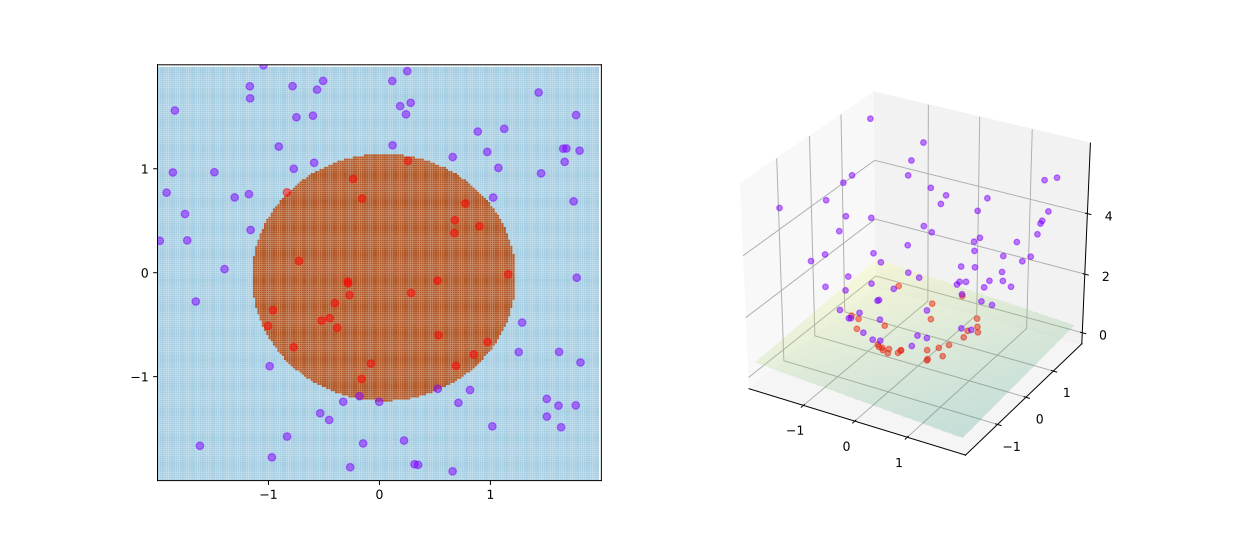
\includegraphics[width=0.6\textwidth]{kerneltrick.png}
  \end{center}
  \vspace{-0.5cm}
  \begin{itemize}
  \item Full (possibly expensive) space transformation can be avoided
    via the \textbf{kernel trick}.\pause
  \item Suppose $\phi(\mathbf{x})$ transforms $x$ into the new space. Kernel
    function $k(\mathbf{x}_i, \mathbf{x}_j) = \phi(\mathbf{x}_i) \cdot \phi(\mathbf{x}_j)$\pause
  \item Now we can can compute dot products for optimization without having the explicit space.
  \end{itemize}
}

\pagestepalt{Kernel functions}{
  Some very basic ones. (They can in
  theory be quite ``bespoke'' to your problem.)
  \begin{itemize}
  \item Polynomial kernel:
    \begin{center}
      $k(\mathbf{x}_i, \mathbf{x}_j) = (\mathbf{x}_i \cdot \mathbf{x}_j)^{d}$
    \end{center}
  \item Radial basis function:
    \begin{center}
      $k(\mathbf{x}_i, \mathbf{x}_j) = \text{exp}(-\gamma\|\mathbf{x}_i - \mathbf{x}_j\|^2)$
    \end{center}
  \end{itemize}
  Often similar to the nonlinearities used in ``real'' neural networks.
}



\end{document}
